
\chapter{Problématisation}\label{chap:problo}
\minitoc
\section{La production audiovisuelle}\label{sec:metier}
% faire le point sur ce que le numérique pourrait apporté à la production audiovisuelle
\e{
L'objectif de cette première section est de donner des éléments de compréhension du métier de la production audiovisuelle.
Dans un premier temps, nous rappelons comment s'organise classiquement la fabrication des objets audiovisuels (\ref{sec:prod}).
Ensuite, nous détaillons les notions et des mots utilisées par les professionnels pour parler de l'objet audiovisuel à construire (\ref{sec:docvoc}).
Enfin, à partir de ces éléments nous précisons les besoins que rencontrent ces professionnels avec l'émergence du numérique et de la mise en réseau (\ref{sec:besoins}). 
}


%%%%%%%%%%%%%%%%%%%%%%%%%%%%%%%%%%%%%%%%%%%%%%%
\subsection{Déroulement de la chaîne de production}\label{sec:prod}
% \addcontentsline{toc}{subsection}{La production audiovisuelle}
La création de documents audiovisuels est une entreprise collective qui suit généralement ce qu'on appelle la chaîne de production audiovisuelle. 
Organisée de manière linéaire, cette chaîne peut se décomposer en 4 grandes étapes -- voir Figure \ref{img:intro:chaine}.

\begin{liste} 
	\item \g{Préproduction} : Cette première étape consiste à construire une ébauche du futur document audiovisuel de manière à prévoir les moyens à engager pour le réaliser.

	\item \g{Production} : Cette étape vise à tourner plusieurs prises pour chaque partie du document et à commencer à faire le tri entre elles.

	\item \g{Postproduction} : L'objectif est d'assembler les prises et de les retoucher de manière à former un document cohérent et adapté à une audience et un mode de distribution.

	\item \g{Exploitation} : Une fois le document achevé, on valorise sa construction par une distribution auprès d'une audience ainsi qu'un archivage qui permettra de le réutiliser ultérieurement.
\end{liste}

\begin{figure}[ht!]
\centering
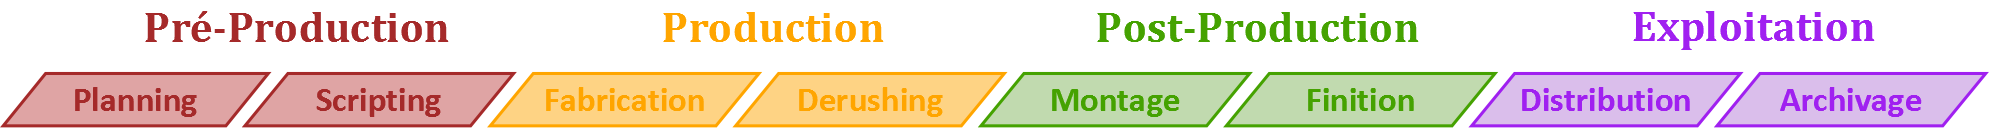
\includegraphics[width=\textwidth]{images/Workflow-Thesis-v0.png}
\caption{La chaîne de production audiovisuelle classique}
\label{img:intro:chaine}
\end{figure}


%%%%%%%%%%%%%%%%%%%%%%%%%
\subsubsection*{Préproduction}\label{sec:preprod}
L'objectif de cette étape est de construire une ébauche du futur document audiovisuel, de manière à prévoir les moyens à engager pour le réaliser. 
On distingue deux phases de préparation, l'écriture ou \e{Scripting} et le \e{Planning} ou planification.

À partir d'une idée, l'écriture du document se déroule en plusieurs étapes où l'on fixe progressivement le message à faire passer ainsi que sa forme audiovisuelle. 
Une fiction par exemple s'écrit à partir d'un résumé de l'histoire, puis on développe les scènes, les personnages, les lieux, les dialogues, etc. jusqu'à arriver à la manière dont cette histoire sera racontée à l'écran. 
On fixe ainsi le type de plan à filmer, les mouvements de caméra, le type de lumière, etc. 
Dans certaines grosses productions, on aura même recours au dessin pour aider à la représentation visuelle.


Toutes ces informations sur le contenu et la forme du futur document audiovisuel servent à estimer le temps nécessaire et les moyens à engager. 
L'estimation du coût d'une production est un élément essentiel pour la production audiovisuelle. 
En effet, dès le départ le producteur doit estimer la rentabilité du futur document afin de voir quels moyens il peut engager. 
Il s'agit bel et bien d'investissement, parfois très lourd, surtout en comparaison avec d'autres industries culturelles – musique, littérature, radio, presse – à l'exception récente du jeu vidéo. 
Contrainte budgétaire et forme esthétique sont donc en négociation dans cette première étape.


%%%%%%%%%%%%%%%%%%%%%%%%%
\subsubsection*{Production}
Une fois l'ébauche et les moyens déterminés, la production vise à réaliser chaque partie du document une à une puis à les assembler en un montage cohérent.

La phase de \e{Fabrication} consiste à capter du réel que l'on a mis en scène. La captation d'un évènement est réalisée grâce à des appareils d'enregistrement (caméra, microphones, etc.). 
La mise en scène du réel se construit à partir d'un ensemble de techniques, d'équipements et d'accessoires (lumière, costume, décors, maquillage, etc.) qui permettent d'obtenir l'image et le son souhaités. 
La technique est ainsi mobilisée dans un objectif esthétique. 
Dans le cas d'une fiction, la fabrication du contenu se fait en fonction du planning de mobilisation des personnes et des équipements plutôt que suivant l'ordre chronologique de l'histoire. 
On regroupe ainsi le tournage des scènes dans tel lieu ou avec tel équipement afin de réduire les coûts. Au final, la fabrication
produit des séquences vidéo et audio qu'il s'agit ensuite de redécouper pour mieux les assembler.

La phase de \e{Derushing} consiste à examiner les séquences réalisées pendant la fabrication et à les trier en vue de faciliter le montage. 
Par exemple, le tournage d'une fiction produit des séquences vidéo comprenant plusieurs prises d'une même scène et souvent des séquences captées par des caméras ayant des angles de prise de vue différents. 
Il faut donc redécouper les séquences en prises puis regrouper les prises d'une même scène. 
Le montage se fera d'autant plus facilement qu'on saura également identifier la qualité et les avantages de chaque prise d'une même scène.


%%%%%%%%%%%%%%%%%%%%%%%%%
\subsubsection*{Postproduction}
Lorsque le contenu audiovisuel est fabriqué et trié, il reste à le structurer en un document et à le conditionner en fonction de sa future exploitation.

La phase de \e{Montage} consiste à agencer des petites séquences de vidéo et d'audio pour construire la structure du document audiovisuel.
L'agencement des plans, leur durée et la transition entre ces plans constituent les ressorts esthétiques propres à l'audiovisuel. 
Ils participent à la transmission du message en ceci qu'ils servent de raccord entre les plans, comme le souligne le réalisateur \pc{Sergueï Mikhaïlovitch Eisenstein}\footnote{L'origine de cette fameuse citation est assez obscur, on la retrouve dans de nombreux documents, dont cet article --\cite{Montage et Réalisme}-- datant des années 60 et extrait de la revue québecoise \gui{Séquence : La revue du cinéma}.} :

\begin{cico}
Le montage est l 'art d'exprimer ou de signifier par le rapport de deux plans juxtaposés de telle sorte que cette juxtaposition fasse naître l'idée ou exprime quelque chose qui n'est contenu dans aucun des deux plans pris séparément. L'ensemble est supérieur à la somme des parties.
\end{cico}

Après le montage, une phase de \e{Finition} est nécessaire pour intégrer d'autres ressources au document en fonction de sa distribution. 
Pour une diffusion antenne d'un reportage, on ajoute le logo de la chaîne de télévision, un jingle, le nom des intervenants ou des titres, etc. 
Une diffusion sur DVD nécessitera l'ajout des conditions
légales d'usages, l'intégration d'un menu de navigation, etc. 
La distribution détermine également un format d'encapsulation (.avi, .mkv, .ogg etc.) et un encodage du contenu audiovisuel (MPEG-2, H.264, MPEG-4, theora vorbis etc.). 
Le résultat de cette phase de post-production est de fournir des documents prêts à l'usage et dans certains cas plusieurs variantes pour chacun des modes de distribution envisagés.


%%%%%%%%%%%%%%%%%%%%%%%%%
\subsubsection*{Exploitation}
Une fois le document achevé, on valorise sa construction par une distribution auprès d'une audience ainsi qu'un archivage qui permettra de le réutiliser ultérieurement.

La phase de \e{Distribution} consiste à rendre le document matériellement accessible à une audience. 
Il s'agit d'un transfert qui peut faire l'objet d'une transaction commerciale ou s'appuyer sur d'autres types de modèles économiques (publicité entre autres). 
La nature du transfert varie et porte à la fois sur les modalités d'accès au contenu et les droits d'usages.

La phase d'\e{Archivage} consiste le plus souvent à stocker le contenu diffusé afin de pouvoir le réutiliser tel quel plus tard, soit en le rediffusant, soit en le vendant à un autre diffuseur. 
C'est aussi généralement la phase où l'on construit, récupère et attache des descriptions du contenu au document audiovisuel. 
En effet, l'archivage n'a de sens que s'il permet de retrouver, voire redécouvrir, les documents archivés.
\ciel{Au plan économique, un film est un bien informationnel, d'expérience, caractérisé par une très forte densité d'informations. Son exploitation s'organise autour de versions différentes, distribuées sur des marchés distincts par des acteurs spécialisés.} (\cite{Blanc2006}).%Gilles Le Blanc - Innovations numériques, distribution et différenciation  : le cas de la projection numérique dans le cinéma.




%<TODO
%TODO>
\subsection{Documents et vocabulaire de la production}\label{sec:docvoc}
\e{
Dans cette section, nous présentons des définitions utilisées dans le milieu professionnel et tirées du \gui{Dictionnaire technique du Cinéma (\cite{Pinel2008})} afin de présenter les principaux documents et le vocabulaire utilisé pendant la phase de préproduction. 
Il s'agit ainsi de mettre en exergue la manière dont se construit une description textuelle de l'objet audiovisuel en devenir ainsi que le vocabulaire utilisé pour faire cette description.}
% Des éléments qui nous serviront à mieux cerner les problèmes qui se posent à la production audiovisuelle.

\paragraph{La notion de plan}
La notion de plan peut se présenter de diverses manières suivant le point de vue adopté. 
Du point de vue technique, il s'agit d'une série d'images (ou photogrammes) qui sont enregistré par un appareil de capatation (une caméra) au cours d'une même prise de vue : \ciel{série de photogrammes enregistrés au cours d'une même prise} (\cite{Pinel2008}).
Il s'agit donc de l'enregistrement qui est effectué entre le moment où l'on presse sur le bouton pour lancer et celui où l'on arrête l'enregistrement.
Cette définition, certes robuste, ne permet pas pour autant de caractériser les plans ou de les comparer entre eux. 
Ainsi, on s'intéresse au point de vue de l'écriture filmique et de la réalisation qui considère non seulement l'action d'enregistrement, mais également la manière dont il est effectué : 

\ciel{
Fragment de temps et d'espace enregistré d'un seul tenant, selon un point de vue déterminé, et donnant à la projection le sentiment de la continuité d'une même \e{image en mouvement}.} (\cite{Pinel2008})

Cette définition complète la précédente en considérant le rapport au sujet (le point de vue) et la temporalité du plan et son rapport à un ensemble d'autres plans (la continuité). 
Elle permet d'envisager les plans comme des éléments de base que l'on assemblera ensuite pour construire un objet audiovisuel : 

\ciel{
La notion de plan est apparue [\dots] lorsqu'on a abandonné le point de vue unique du tableau pour envisager le sujet sous différents angles et à différentes distances et lorsque, par la grâce du montage, on a mis en relation ces plans entre eux.
[\dots]
Si le photogramme représente l'unité technique de la prise de vues, la scène et la séquence les unités narratives de l'oeuvre cinématographique, le plan est la cellule fondamentale de l'écriture du film, de sa préparation jusqu'à la copie standard.} (\cite{Pinel2008})

Dans cette citation, on voit aussi émerger l'idée qu'il existe différents niveaux d'analyse dans l'objet audiovisuel : 
\begin{liste}
	\item un \g{niveau technique} avec le photogramme mais également le pixel dans le numérique.
	\item un \g{niveau narratif} avec la scène (unité de temps et de lieu dans l'histoire) et la séquence (suite de scènes constituant une action dramatique autonome ou distincte).
	\item \g{un niveau dont le plan est l'unité de base qui sert tout au long de la chaîne de production}. 
	On parle d'unité, car il s'agit du résultat de base d'une prise de vue, c'est-à-dire de la fabrication (production) de l'objet audiovisuel. 
	La pré-production, étape de préparation du tournage, utilise donc naturellement cette unité. 
	De même, le montage consiste à organiser ces plans pour former un ensemble cohérent, quitte à les ajuster (raccourcir, allonger, modification du cadrage etc.). 
	Ainsi, il semble que cette unité servent non seulement d'unité de travail de référence pour la chaîne de production\footnote{La production sonore d'un objet audiovisuel ne s'organise pas forcément de la même manière que celle de la production de l'image. Néanmoins, par la force des choses, la construction de l'image prime bien souvent sur celle du son et son unité de base sert donc de référence même pour la production sonore.}, mais également du premier niveau signifiant propre à l'audiovisuel (l'image seul pouvant être rattaché à la photographie).
\end{liste}

Ces distinctions nous permettent de définir le plan selon les caractéristiques suivantes : 
\begin{liste}
	\item \g{l'échelle relative du cadre par rapport au(x) sujet(s)} (personnages, objets etc.).
	C'est ce qui permet de définir un ensemble de \gui{valeurs de plan}, gros plan, plan américain etc. que nous définirons par la suite.
	
	\item \g{l'angle de la prise de vue} (plongée, contre-plongée, cadre incliné etc.)

	\item \g{le mouvement de la caméra} et d'autres paramètres de son objectif (panoramique, travelling, rotation, zoom, focale, focus etc.)

	\item \g{l'articulation des plans entre eux}, d'une part en terme de durée, mais aussi en terme de transition et d'impression de continuité entre les plans. 
	Par exemple, il existe des règles de cadrage et de montage pour aider les spectateurs à situer les personnes sur un plateau\footnote{La règle des 180° oblige ainsi à maintenir les mêmes relations est-à-gauche/droite-de entre les personnes, de manière à ce que le spectateur puisse se souvenir des positions des interlocuteurs sur un plateau. En inversant ces relations topographiques, on donne l'impression au spectateurs que les personnes ont échangé leurs places alors que c'est juste la caméra qui a changé de point de vue. Il s'agit donc d'une règle très importante pour assurer la continuité et la compréhension du spectateur.}.
\end{liste}


\paragraph{Valeurs de plan utilisées dans un script}
La valeur de plan est un des éléments le plus utilisé pour distinguer les plans entre eux, notamment au moment de l'écriture. 
Plutôt que de préciser les paramètres optiques de la caméra (considérés comme des détails très difficile à préciser à l'avance), le réalisateur préfère parler d'un type de plan pour donner une idée générale de l'image à obtenir. 
Le Tableau \ref{tab:vplans} présente les principales valeurs de plans utilisées par les professionnels, avec leur abréviations et leur(s) dénomination(s) anglaise(s) tandis que la Figure \ref{img:intro:plans} en propose une illustration.

\begin{table}[ht!]
   \begin{center}
		\begin{tabularx}{\textwidth}{|p{100pt}|X|p{100pt}|}
		   \hline
	\pc{Dénomination française} & \pc{Défintion} & \pc{Dénomination anglaise} \\ \hline\hline
 	\g{très gros plan (t.g.p.)} & plan cadrant une partie du visage, un détail du corps (un oeil, une bouche, un doigt etc.) ou le détail d'un objet. & extreme close-up, e.c.u. ; big close-up, b.c.u.\\ \hline

 	\g{gros plan (g.p.)} & plan isolant un visage, généralement cadré à la hauteur du noeud de cravate, ou un autre détail du corps (plan de détail ; insert), voire \e{tout ou partie d'un petit objet}. & close-up, c.u.\\ \hline

	\g{plan rapproché} & plan cadrant le(s) personnage(s) au niveau de la taille (plan rapproché taille, p.r.t.) ou de la poitrine (plan rapproché poitrine, p.r.p.). & medium close-up, m.c.u.\\ \hline
	
	\g{plan ceinture} & plan coupant les personnages au niveau de la ceinture & belt shot\\ \hline 

	\g{plan américain} (p.a.) & plan coupant les personnages à mi-cuisse & american shot ; medium close-shot, m.c.s.\\ \hline
	
	\g{plan moyen (p.m.) ou plan en pied} & plan présentant le(s) personnage(s) en pied. Il existe également des variations de ce plan qui sont nommées \e{serré} (aussi nommé plan américain large) ou \e{large} et qui font varier légèrement le cadrage. & medium shot, middle-shot, mid-shot, m.s. ; full shot, f.s.\\ \hline
	

	\g{plan de demi-ensemble (p.d.e., 1/2e.)} & plan mettant en place les personnages dans leur milieu en cadrant une bonne partie du décor & medium-long shot, m.l.s.\\ \hline

	\g{plan d'ensemble (p.e.)} & plan cadrant l'ensemble du décor construit & long shot, l.s.\\ \hline
	
	\g{plan de grand ensemble (p.g.e.)} & plan cadrant l'ensemble du décor construit de grande envergure. & very long shot, v.l.s.\\ \hline

	\g{plan général (p.g.)} & plan couvrant un vaste ensemble qui situe le décor construit dans son cadre : le décor dans le décor. & master shot ; extreme long shot, e.l.s\\ \hline 
		\end{tabularx}
		\caption{Valeurs de plans : du plus précis au plus général \label{tab:vplans}}
   \end{center}
\end{table}

% \begin{liste}
% 	\item \g{très gros plan} (t.g.p.) : \ciel{plan cadrant une partie du visage, un détail du corps (un oeil, une bouche, un doigt etc.) ou le détail d'un objet}. [extreme close-up, e.c.u. ; big close-up, b.c.u.]

% 	\item \g{gros plan} (g.p.) : \ciel{plan isolant un visage, généralement cadré à la hauteur du noeud de cravate, ou un autre détail du corps} (plan de détail ; insert), voire \ciel{tout ou partie d'un petit objet}. [close-up, c.u.]

% 	\item \g{plan rapproché} : \ciel{plan cadrant le(s) personnage(s) au niveau de la taille (plan rapproché taille, p.r.t.) ou de la poitrine (plan rapproché poitrine, p.r.p.).} [medium close-up, m.c.u.]
	
% 	\item \g{plan ceinture} : plan coupant les personnages au niveau de la ceinture [belt shot] 

% 	\item \g{plan américain} (p.a.) : \ciel{plan coupant les personnages à mi-cuisse} [american shot ; medium close-shot, m.c.s.]
	
% 	\item \g{plan moyen} (p.m.) ou \g{plan en pied} : \ciel{plan présentant le(s) personnage(s) en pied.} [medium shot, middle-shot, mid-shot, m.s. ; full shot, f.s.]
% 	Il existe également des variations de ce plan qui sont nommées \ciel{serré} (aussi nommé plan américain large) ou \ciel{large} et qui font varier légèrement le cadrage.

% 	\item \g{plan de demi-ensemble} (p.d.e., 1/2e.): \ciel{plan mettant en place les personnages dans leur milieu en cadrant une bonne partie du décor}. [medium-long shot, m.l.s.]

% 	\item \g{plan d'ensemble} (p.e.) : \ciel{plan cadrant l'ensemble du décor construit}. [long shot, l.s.]
	
% 	\item \g{plan de grand ensemble} (p.g.e.) : \ciel{plan cadrant l'ensemble du décor construit de grande envergure}. [very long shot, v.l.s.]

% 	\item \g{plan général} (p.g.) : \ciel{plan couvrant un vaste ensemble qui situe le décor construit dans son cadre : le décor dans le décor}. [master shot ; extreme long shot, e.l.s] 
% \end{liste}
%TODO:source

\begin{figure}[ht!]
\centering
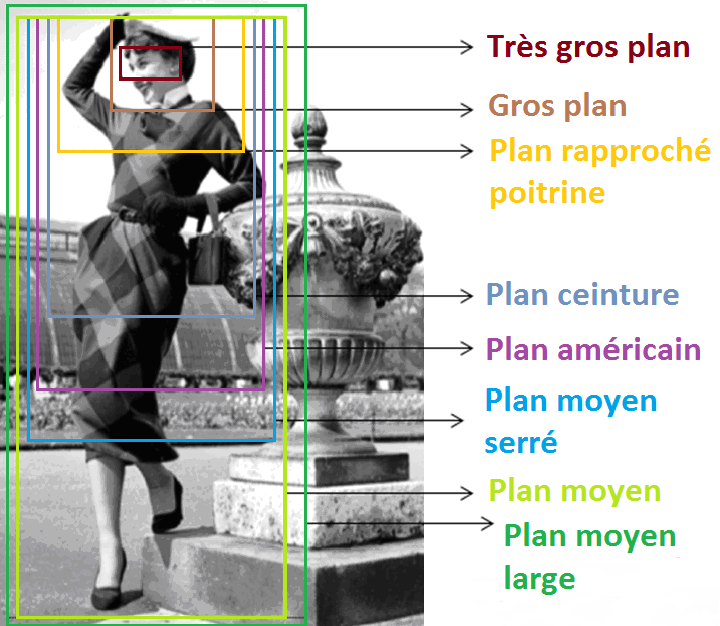
\includegraphics[width=0.4\textwidth]{./images/ValeurPlan-v1.png}
\caption{Différentes valeurs de plan pour le cadrage d'un personnage à l'écran}
\label{img:intro:plans}
\end{figure}


\paragraph{Quelques documents de (pré)production}
%TODO:description + source
La pré-production se repose sur différents types de documents qui permettent de faire émerger progressivement la structure narrative ou documentaire, le découpage en plans et tous les détails de réalisation nécessaire à une bonne préparation du tournage. 
On notera que chacun de ces documents constitue un jalon dans la préparation du projet et que le script, résultat final de cette écriture, constitue une sorte de cahier des charges de l'objet audiovisuel à fabriquer.
\begin{liste}
	\item \g{sujet} : \ciel{matière première du film enrichie et développée lors de la préparation puis mise en forme au cours de la réalisation et du montage.} 
	
	\item \g{synopsis} : \ciel{exposé sommaire en quelques lignes, voire en quelques pages, du contenu dramatique ou documentaire d'un film}. 
	À noter que ce document est également utilisé plus tard dans la chaîne de production, notamment pour être transmis aux journalistes ou aux archivistes.
	De plus, il constitue la première mise en forme narrative du contenu du film, à la différence du sujet qui ne se constitue que de quelques idées directrices. 

	\item en cas d'adaptation d'une oeuvre littéraire en un objet audiovisuel, on développe un \g{traitement} : 
	\ciel{Travail littéraire préparatoire effectué à partir d'une oeuvre pré-existante ou d'une oeuvre originale pour assurer sa transmutation en termes cinématographiques.}

	\item lorsqu'on développe un objet audiovisuel original, à défaut de traitement on peut parler de \g{scénario} :
	\ciel{description de l'action d'un film épousant la forme \e{littéraire} du récit, rendant compte des articulations narratives et comportant une ébauche des dialogues, quelquefois la description plus précise de certaines scènes-clefs.}

	\item lorsque le besoin de préciser encore la construction de la narration, les auteurs peuvent construire une \g{continuité (dialoguée)} : \ciel{étape de la préparation écrite du film qui permet d'enrichir le traitement en développant chronologiquement les fragments d'action, en mettant au point le détail de chaque scène et en précisant le dialogue.}

	\item \g{plan de tournage} : \ciel{ultime travail de préparation effectué par le réalisateur avant le tournage. Il consiste à fragmenter la continuité en unités cinématographiques de temps et d'espace : les plans.}

	\item \g{script} : \ciel{dernière mouture du scénario, guide complet du tournage}.La Figure \ref{img:intro:script} présente un exemple de script extrait d'un film récent écrit et réalisé par Quentin Tarantino.
\end{liste}

\begin{figure}[ht!]
\centering
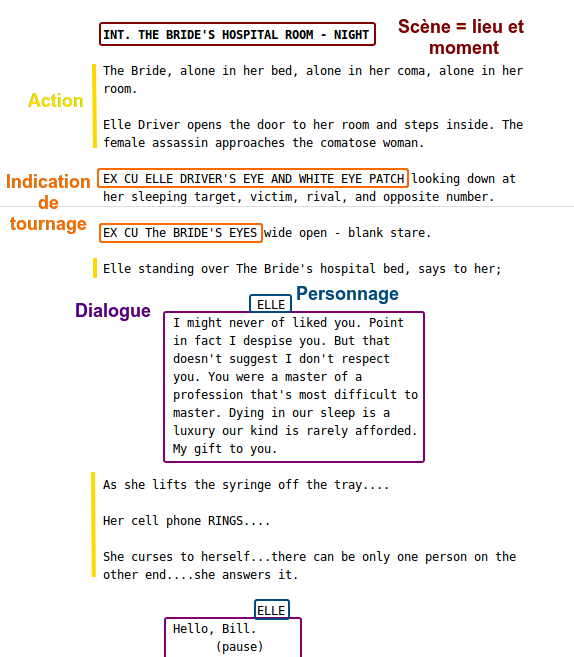
\includegraphics[width=0.7\textwidth]{images/ScriptExample-v1.png}
\caption{Extrait du script de Kill Bill écrit et réalisé par Quentin Tarantino}
\label{img:intro:script} 
\end{figure}

% des réécritures de documents et des mises à jours qui pourraient être réalisées par des machines, des informations qui pourraient être transmises automatiquement à travers un réseau numérique d'information


% un vocabulaire bien défini qui fait l'objet de nombreux dictionnaires, donc prêt à être formalisé


% des équipes qui sont réduites lors de tournage en extérieur



